\begingroup
\setlength{\fboxsep}{10pt}%
% Setting up the verbatim boxes with code examples.
\def\linenumber{%
  \parbox{8pt}{%
    \footnotesize
    \raggedleft
    \textnormal{\arabic{VerbboxLineNo}}%
  }%
  \hspace{5pt}%
}%
\verbfilebox[\linenumber\small]{images/iceberg-code-01.tex}%
\newsavebox\firstcode\sbox\firstcode{\box\savedverbbox}%
\begin{tikzpicture}[every node/.style={inner sep=0pt, outer sep=0pt}]
% The iceberg in the background
\node (background) at (0, 0) {{%
  \transparent{0.2}%
  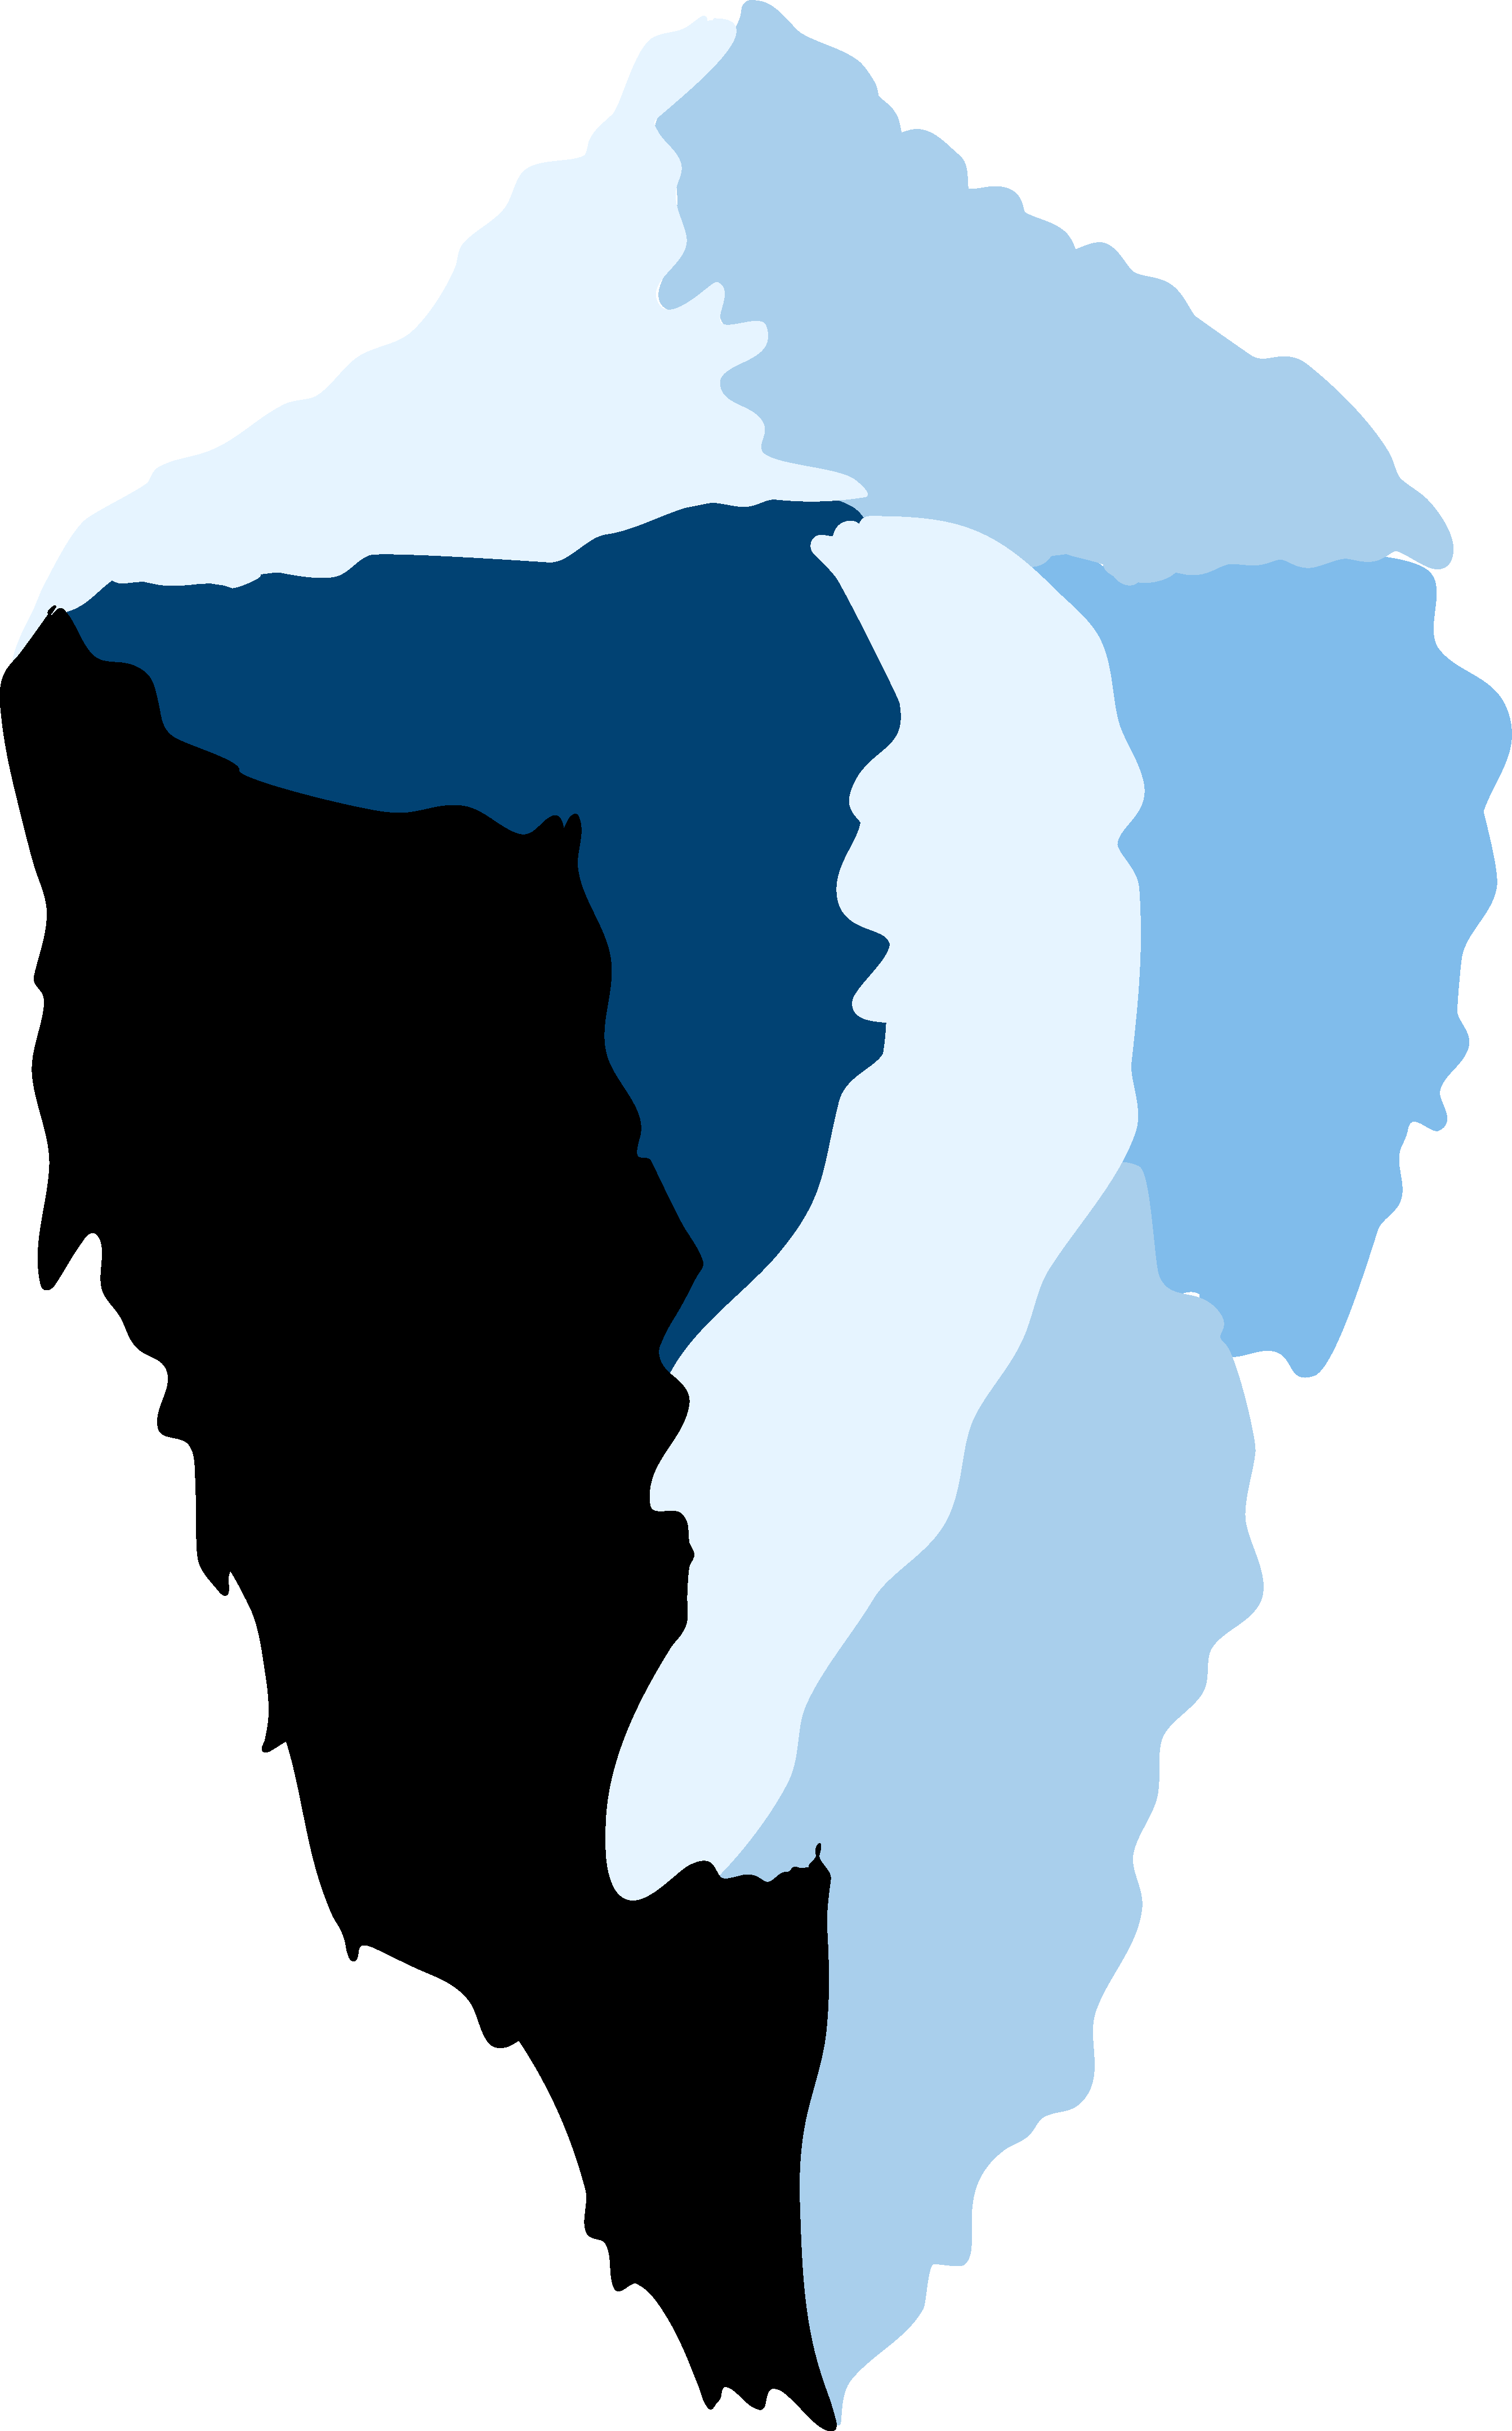
\includegraphics[width=0.7\linewidth]{images/iceberg-color}%
}};
% The water surface
\draw[decorate, decoration={snake, segment length=15.05mm, amplitude=2mm}] (-10, 5) -- (6, 5);
% The LaTeX source code as an abstract ice floe
\node [left=of background.north, xshift=0.5cm, yshift=-1.5cm, rotate=1] (code-01-tex) {%
  \fcolorbox{black}{white}{\usebox{\firstcode}}%
};
% The result of compiling the source code as another ice floe
\node [right=of code-01-tex.south east, anchor=south west, xshift=1cm, rotate=-1] (code-01-pdf) {%
  \fcolorbox{black}{white}{%
    \includegraphics[width=3cm]{images/iceberg-code-01}%
  }%
};
% The compilation, i.e. the "above-the-surface" of a TeX document.
\draw [-{Stealth[length=3mm, width=3mm]}, line width=\fboxrule] ([xshift=5pt] code-01-tex.east) to [bend left] node [text width=5cm, midway, above, align=center, rotate=-10, xshift=1cm, yshift=0.5cm] {%
  compile with\\
  \texttt{lualatex example.tex}%
} ([yshift=5pt] code-01-pdf.north);
\end{tikzpicture}
\endgroup
\vspace{0.75cm}%